\documentclass[border=10pt]{standalone}

\usepackage{tikz}
\usepackage{tikzsymbols}
\usetikzlibrary{calc,patterns,shapes.geometric}

\def\centerarc[#1](#2)(#3:#4:#5){\draw[#1] ($(#2)+({#5*cos(#3)},{#5*sin(#3)})$) arc (#3:#4:#5);}

\begin{document}
	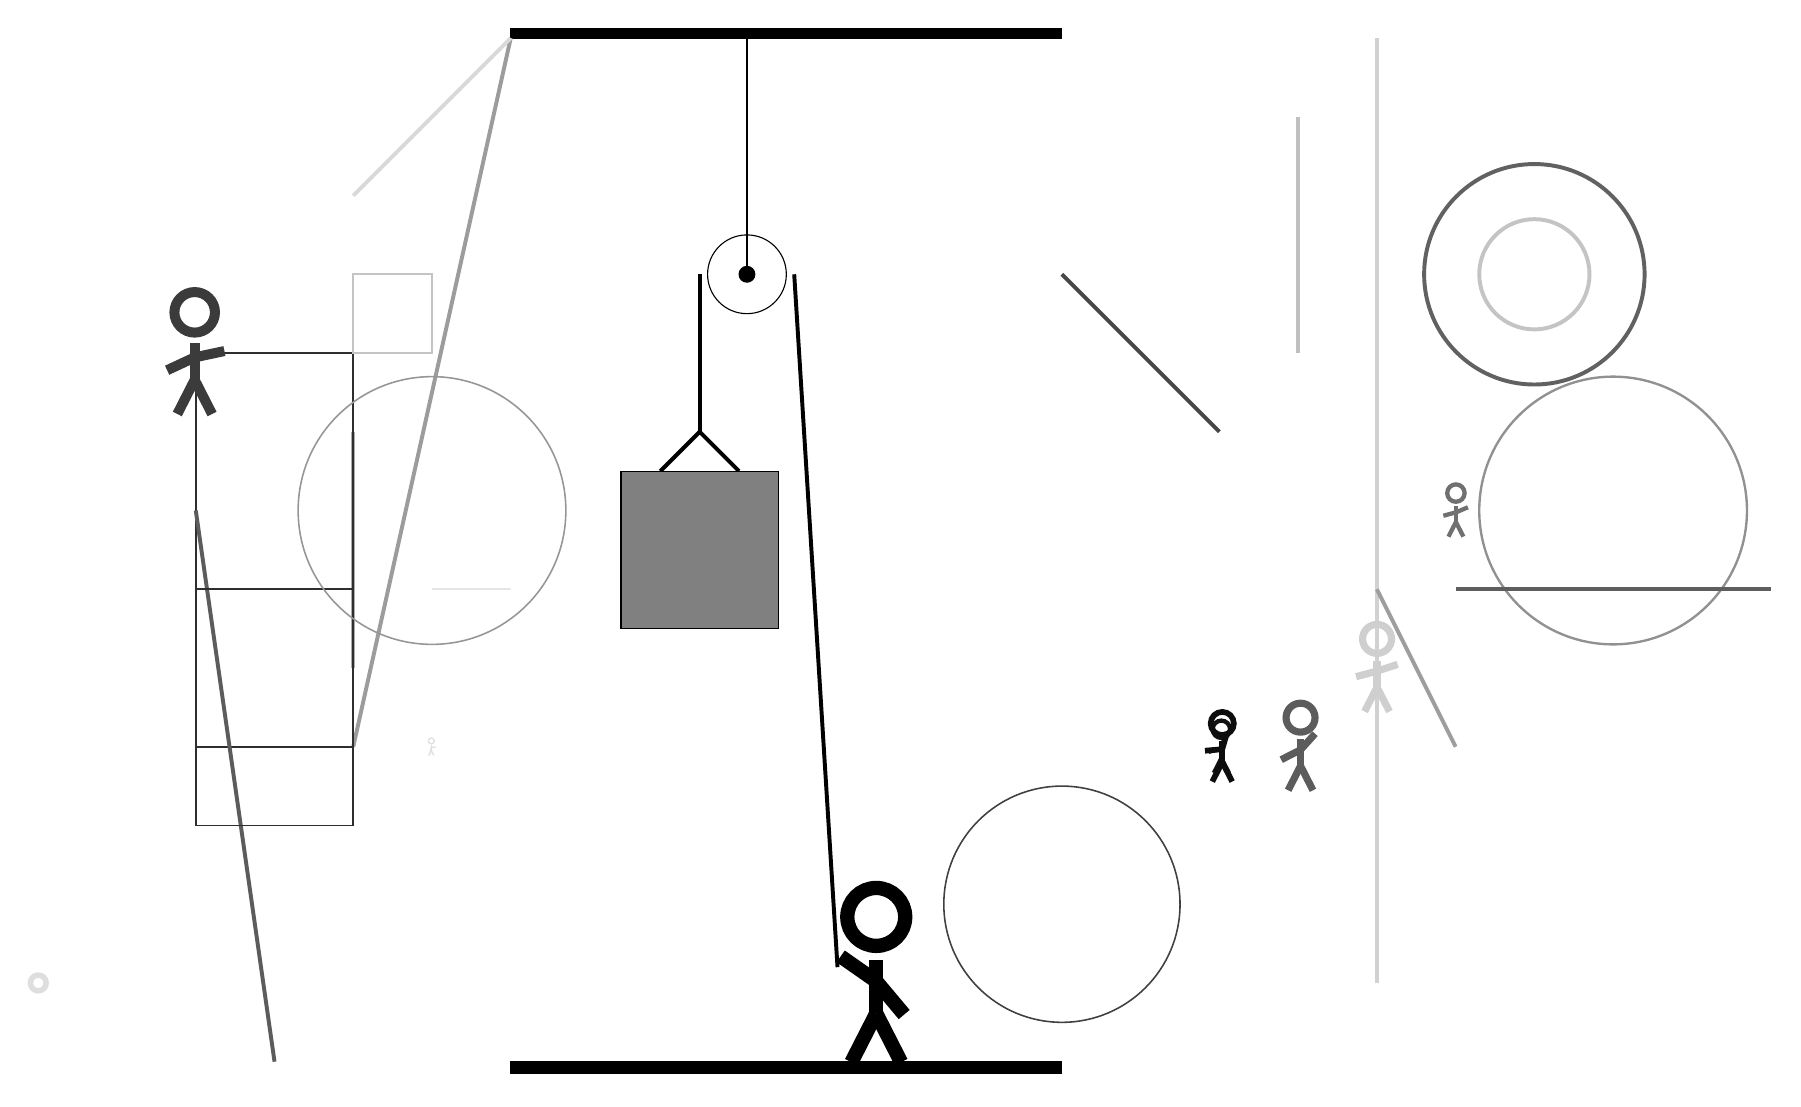
\begin{tikzpicture}
		%%%%% START %%%%%
		
		\draw[fill=black] (-2, 10) rectangle (5, 10.125);
		
		\draw (1, 7) circle (0.5);
		\draw[fill=black] (1, 7) circle (0.1);
		\draw (1, 10) -- (1, 7);
		
		\draw[line width=0.5mm] (-0.1, 4.5) -- (0.4, 5.0) -- (0.9, 4.5);
		\draw[fill=black!50] (-0.6, 4.5) rectangle (1.4, 2.5);
		
		\draw[line width=0.5mm] (0.4, 7) -- (0.4, 5.0);
		\centerarc[line width=0.5mm](1, 7)(0:180:0.6);
		\draw[line width=0.5mm](1.6, 7) -- (2.15, -1.8);
		
		\draw[line width=0.5mm, color=black!32](-4, 2) -- (-4, 5);
		
		\draw[line width=0.5mm, color=black!39](-4, 1) -- (-2, 10);
		\node[line width=0.2mm, color=black!64] at (8, 1) {\Strichmaxerl[5][27][48]};
		\draw [line width=0.5mm, color=black!23](11, 7) circle (0.7);
		\draw[line width=0.5mm, color=black!72](7, 5) -- (5, 7);
		\draw[line width=0.5mm, color=black!15](-2, 10) -- (-4, 8);
		\draw[line width=0.5mm, color=black!25](8, 6) -- (8, 9);
		
		\draw[line width=0.3mm, color=black!82] (-4, 1) rectangle (-6, 6);
		\draw [line width=0.2mm, color=black!75](5, -1) circle (1.5);
		
		\node[line width=0.5mm, color=black!56] at (10, 4) {\Strichmaxerl[3][15][23]};
		
		\draw[line width=0.5mm, color=black!64](-5, -3) -- (-6, 4);
		\draw[line width=0.5mm, color=black!18](9, 10) -- (9, -2);
		\draw [line width=0.5mm, color=black!62](11, 7) circle (1.4);
		
		\draw[line width=0.2mm, color=black!10] (-3, 3) rectangle (-2, 3);
		\node[line width=0.4mm, color=black!93] at (7, 1) {\Strichmaxerl[3][14][73]};
		\draw[line width=0.2mm, color=black!82] (-4, 0) rectangle (-6, 3);
		\node[line width=0.6mm, color=black!77] at (-6, 6) {\Strichmaxerl[7][25][12]};
		\draw [line width=0.7mm, color=black!13](-8, -2) circle (0.1);
		\draw[line width=0.5mm, color=black!38](10, 1) -- (9, 3);
		\draw[line width=0.2mm, color=black!23] (-4, 7) rectangle (-3, 6);
		\node[line width=0.3mm, color=black!19] at (9, 2) {\Strichmaxerl[5][15][18]};
		
		\draw [line width=0.3mm, color=black!43](12, 4) circle (1.7);
		\node[line width=0.3mm, color=black!12] at (-3, 1) {\Strichmaxerl[1][76][4]};
		\draw[line width=0.5mm, color=black!63](10, 3) -- (14, 3);
		\draw [line width=0.2mm, color=black!41](-3, 4) circle (1.7);
		\node[line width=0.6mm, color=black!95] at (7, 1) {\Strichmaxerl[4][5][74]};
		
		
		\node at (2.6, -1.9) {\Strichmaxerl[10][-35][-50]};
		
		\draw[fill=black] (-2, -3) rectangle (5, -3.15);
		
		%%%%% END %%%%%
	\end{tikzpicture}
\end{document}